
\chapter{Self-Calibration of Coded Illumination Systems}\label{ch:selfcal}

In Chapter~\ref{ch:introduction}, we described a general computational imaging framework which consisted of both a forward model generation step as well as a computational inversion. In all imaging systems, the forward model is synthesized from the fundamental laws of light propagation (e.g. Maxwell's equations), the optical design of the system, and the accumulated error from optical mis-alignment, dust, manufacturing imperfections, and other sources which can be collectively referred to mis-calibration. While some of these imperfections can be removed using simple processes (such as background subtraction), others, such as system aberrations, are relatively complex, and need to be tolerated or removed using a more sophisticated procedure.

\section{Algorithmic Self-Calibration}
The concept of algorithmic self-calibration (solving jointly for the reconstructed image and the calibration parameters) has proven particularly useful in coherent computational imaging. Examples include probe retrieval in Ptychography~\cite{guizar2008phase, maiden2009improved, tripathi2014ptychographic, Maiden2012}, source recovery for through-focus phase imaging~\cite{jingshan2015partially, zhong2016nonlinear}, pupil and source recovery for Fourier Ptychography Microscopy (FPM)~\cite{Bian:13,Yeh2015,Bian:16}, and calibration-invariant inverse scattering models~\cite{satat2017object}. The standard approach to self-calibration uses alternating projections (AP), which optimizes multiple variables serially, keeping other parameters fixed during each sub-iteration. The non-convexity of AP provides no guarantee of global convergence, but in practice it works with sufficiently diverse data. Self-calibration of aberrations has been demonstrated previously in an LED array microscope for the cases of through-focus phase~\cite{zheng2013characterization} and FPM~\cite{Bian:13,Horstmeyer:14,Ou:14,tian2015computational,Chung:16fluor}, but required a large number of images to be captured. For example, a typical FPM setup~\cite{ou2015high} uses approximately 5$\times$ as many images as our system to achieve the equivalent resolution.

Mathematically, a forward model $\op{A}\{\cdot\}$ can be made a function of any variable, including an arbitrary calibration vector $\vec{c}$, with a simple modification of Eq.~\ref{eq:intro_forward_model}:

\begin{equation}\label{eq:self_calib_forward}
    y = \vec{A}\{\vec{x}; \vec{c}\} + \vec{\eta}
\end{equation}

In the case where $\op{A}$ is differentiable with respect to $\vec{c}$, it becomes possible to recover $\vec{c}$ with knowledge of $\vec{x}$ through direct inversion or gradient methods, though this is only very rarely the case. When $\vec{x}$ is unknown, it becomes necessary to solve for both $\vec{x}$ and $\vec{c}$ using an alternating minimization. When $\vec{c}$ is the point spread function of the system (convolution kernel), this becomes a blind deconvolution problem, which has been extensively studied in both microscopy~\cite{Holmes1992blind, sarder2006deconvolution} and photography~\cite{ayers1988iterative, bell1995information, chan1998total, levin2006blind}. However, $\vec{c}$ can also represent system aberrations~\cite{Ou:14}, illumination parameters such as LED positions~\cite{Yeh2015}, or other parameters.

When $\op{A}$ is differentiable with respect to both $\vec{x}$ (the object) and $\vec{c}$ (the PSF), it can be solved by taking the gradient with respect to $\vec{c}$ and $\vec{x}$ in alternating steps. So long as each gradient step is not too large (or is optimized locally using a line search), this alternating minimization technique will not diverge, and will only improve the initial estimate of $\vec{x}$ and $\vec{c}$ until convergence. However, this alternating approach is non-convex, and therefore is very sensitive to initialization since there are many local minima.

\section{Aberration Self-Calibration using Differential Phase Contrast}\label{sec:selfcal:dpc}

System aberrations are nearly always present in optical systems, and may be field-dependent in some cases (such as low-magnification objectives). When performing DPC, these aberrations can corrupt reconstructions due to model mis-match, especially at high frequencies. It is well-known that aberrations arising from optical mis-alignments can be mostly classified by a small number of Zernicke Polynomials~\cite{ZERNIKE1934689}, which makes these functions particularly well-suited for self-calibration.

In this section, we propose a method of algorithmic self-calibration for Differential Phase Contrast (DPC) microscopy~\cite{kachar1985asymmetric,mehta2009quantitative,tian2015quantitative,Claus2015,chen20163d,PhillipsChen17cDPC}, where we avoid the need for pre-calibration by jointly recovering both the sample's complex-field \textit{and} the spatially-varying aberrations of the system, directly from raw images\footnote{This work was developed in close collaboration with fellow Ph.D. student Michael Chen (Waller Lab, EECS, UC Berkeley).}. The method is an extension of illumination-based DPC microscopy~\cite{mehta2009quantitative,tian2015quantitative}, where images are captured with different source patterns, then a reconstruction algorithm recovers the complex-field. Experiments are implemented in a commercial brightfield microscope with a low-cost programmable LED array light source, such that patterns can be switched quickly with no moving parts~\cite{Zheng2013,Liu2014,tian2015quantitative,tian2015computational}. Among the wide variety of QPI methods, those which use partially coherent illumination, like DPC, are advantageous since they provide 2$\times$ better resolution, more light throughput and reduced speckle~\cite{Wang2011,rodrigo2014rapid,jingshan2015partially,tian2015quantitative}, as compared to coherent methods.


To efficiently recover both the complex field and system aberrations, we employ an AP framework that uses 4 captured images for simultaneous phase retrieval and digital correction of spatially-varying aberrations (Fig.~\ref{fig:self_cal_dpc_joint_estimation}). Three of the measurements are partially-coherent conventional DPC images (with rotated half-circle sources); these provide good phase contrast, but poor aberration contrast. The fourth image uses single-LED (spatially coherent) illumination; this provides aberration contrast, but alone cannot resolve the ambiguity between complex-field and pupil aberration~\cite{lu2016quantitative}. Using both partially-coherent and coherent images together improves sensitivity to aberrations without sacrificing the benefits of partial coherence. We model the aberrations parametrically (with a Zernike basis~\cite{ZERNIKE1934689, zheng2013characterization}) to dramatically reduce the number of unknowns. In addition, by segmenting the field-of-view (FOV), we are able to recover and digitally correct for spatially-varying aberrations across the FOV.

\begin{figure}[ht!]
\centering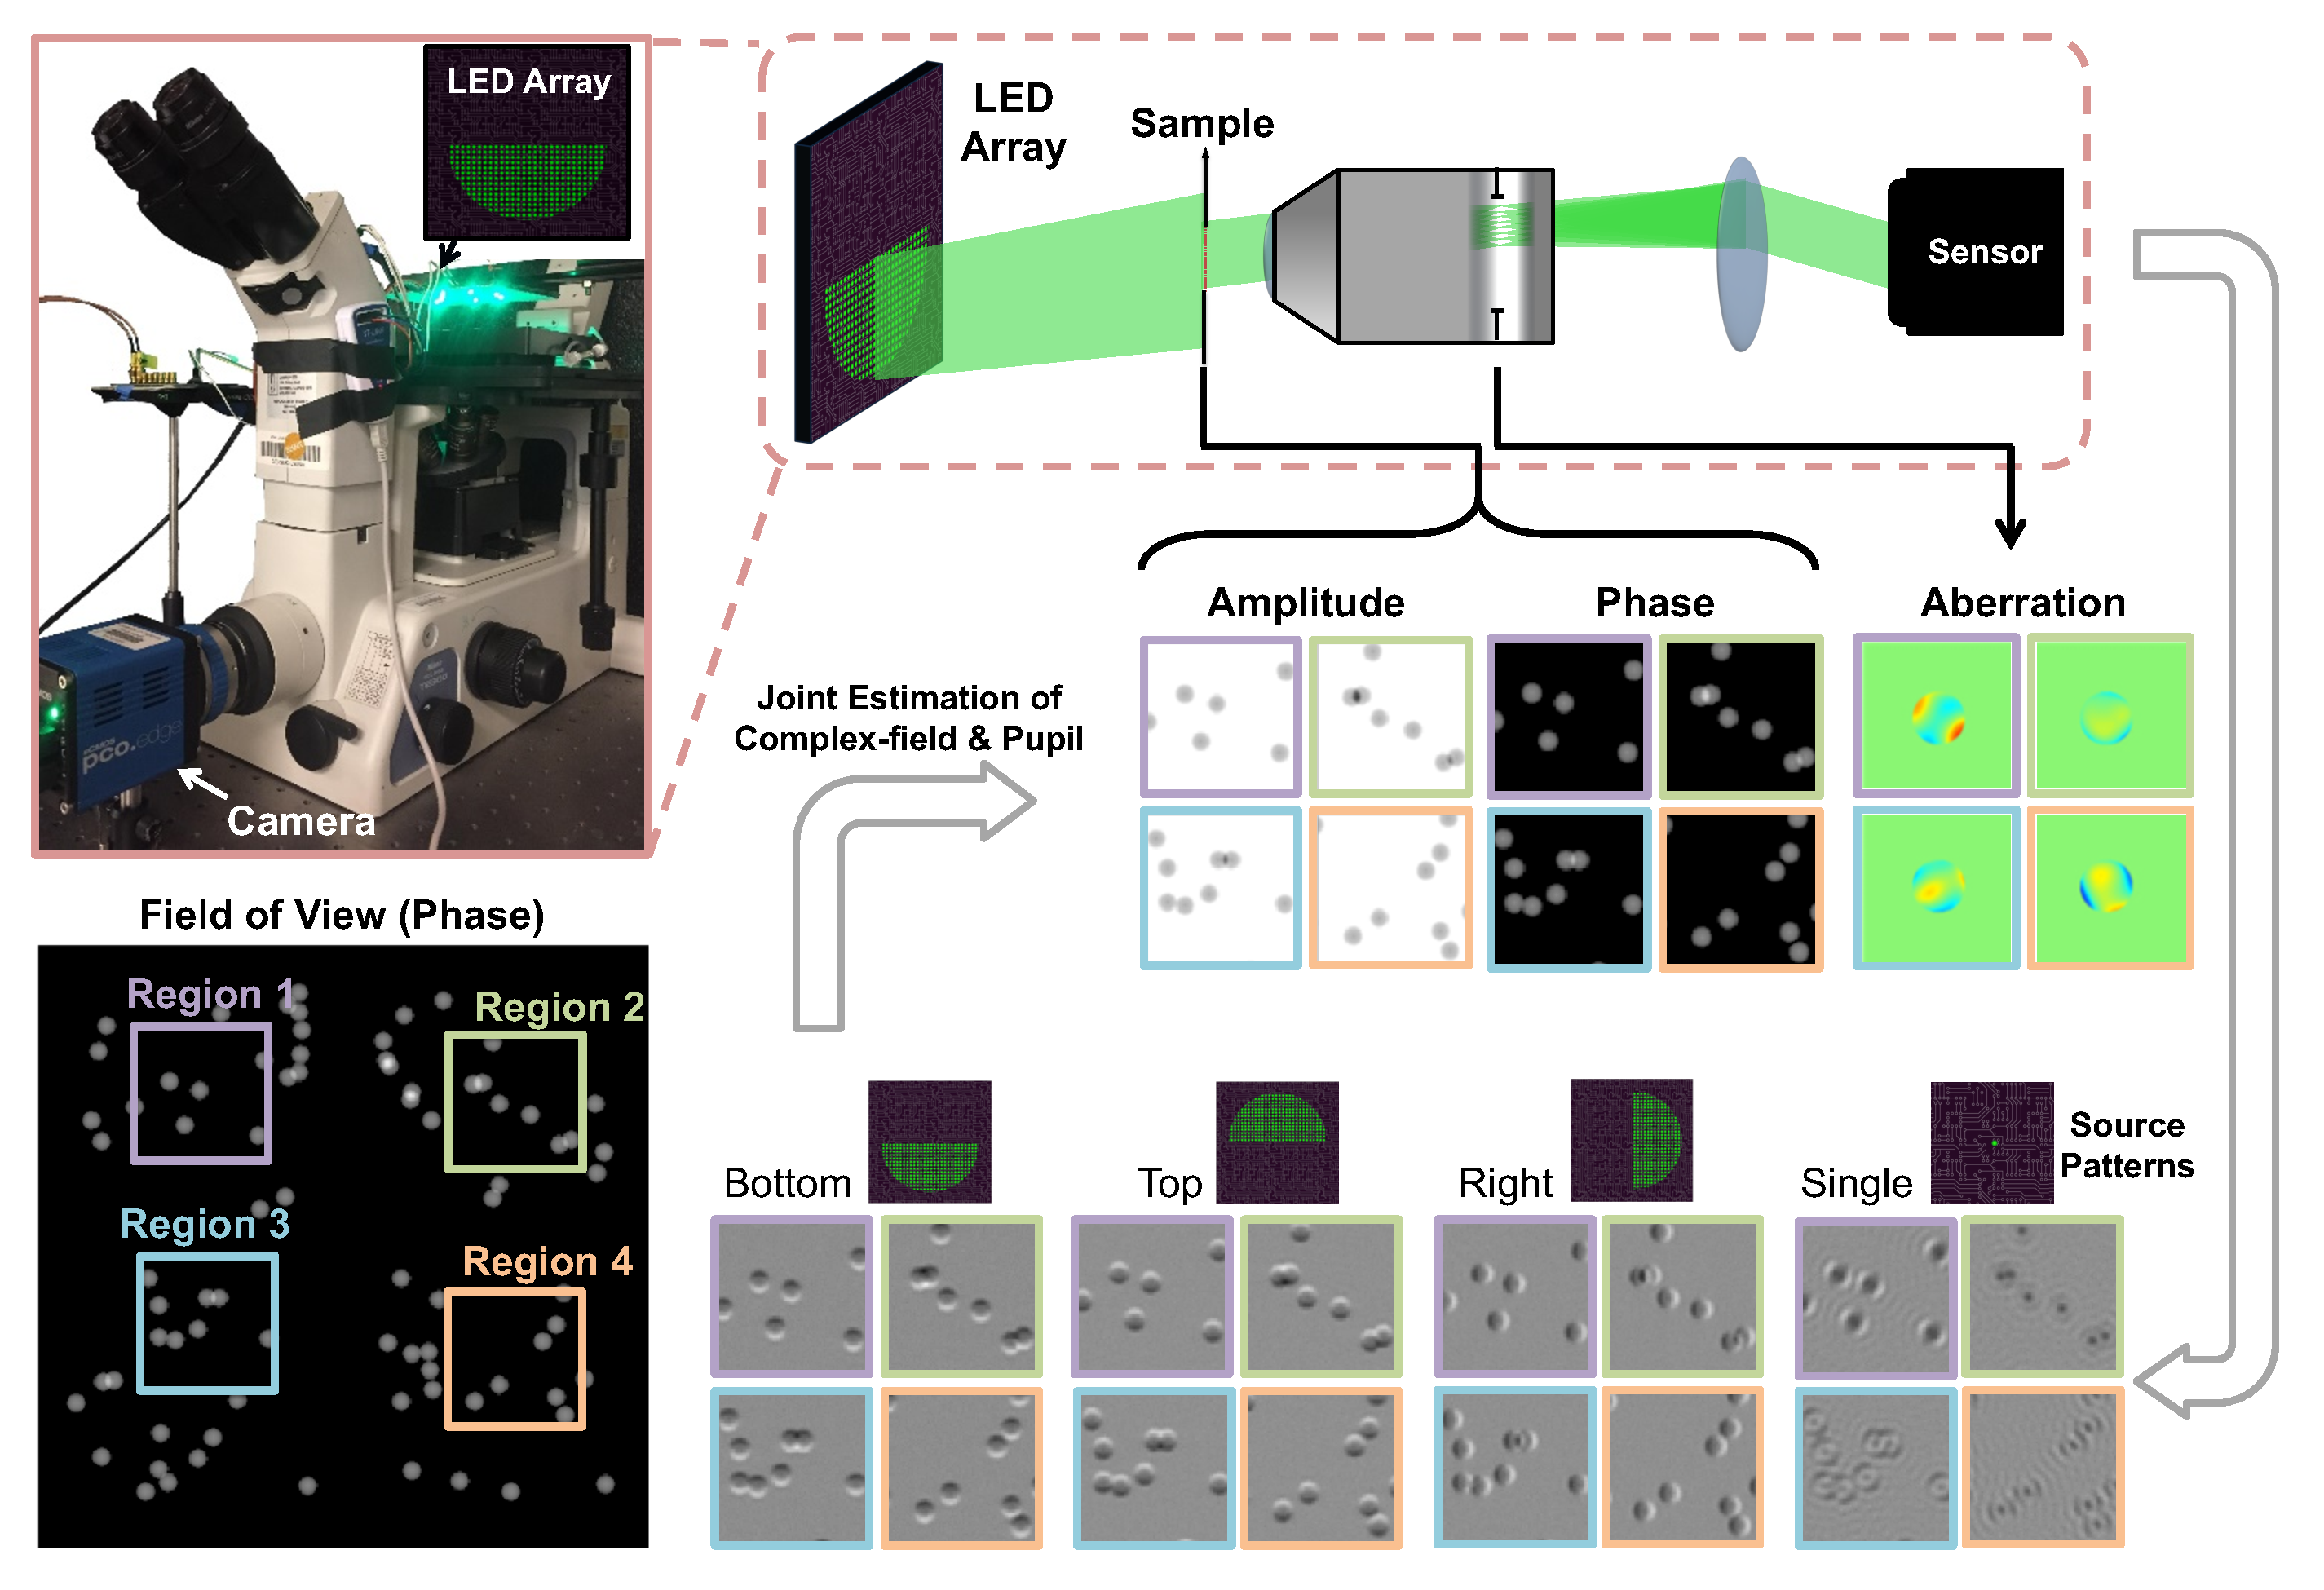
\includegraphics[width=0.9\textwidth]{fig_self_cal_dpc_joint_estimation.pdf}
\caption{\label{fig:self_cal_dpc_joint_estimation} Our LED array microscope captures 4 images with different illumination source patterns (three half-circles and one single LED). The intensity images are used to simultaneously reconstruct both amplitude and phase of the sample, and to estimate the pupil aberrations at each spatial location, which are then digitally corrected for. We show reconstructions for 4 regions with different spatially-varying aberrations.}
\end{figure}

\subsection{Joint Estimation of Complex-Field and Aberrations}

Our LED array microscope and data capture scheme is shown in Fig.~\ref{fig:self_cal_dpc_joint_estimation}. Quantitative DPC (without aberration correction) requires a minimum of 3 intensity measurements to reconstruct phase~\cite{PhillipsChen17cDPC}, though only two quantities (amplitude and phase) are reconstructed at each pixel. Hence, there is significant redundancy in the data which may, in principle, be used to solve for aberrations. Unfortunately, intensity images formed by partially-coherent illumination do not exhibit significant aberration contrast. Hence, we modify the capture scheme to add one additional measurement with spatially-coherent illumination (a single on-axis LED). The example in Fig.~\ref{fig:self_cal_dpc_joint_estimation} has a different aberration in each quadrant of the FOV, and only the single-LED image displays visible differences in contrast for each region. An off-axis LED would also provide the necessary coherent contrast, but the on-axis LED provides higher intensity and better signal-to-noise ratio (SNR). Having achieved both phase and aberration contrast with 1 on-axis and 3 half-circle sources, we use this dataset to jointly recover both spatially-varying aberrations and the complex-field of the sample (with resolution set by the incoherent diffraction limit).

The process of estimating the sample's complex-field and the system's aberrations simultaneously is a joint estimation large-scale nonlinear non-convex problem. To simplify, DPC typically makes a weak scattering approximation which linearizes the forward model. This approximation is generally valid for optically thin or index-matched samples, like biological cells. Intensity measurements can then be related to absorption ($\vec{\mu}$) and phase ($\vec{\phi}$) of the sample~\cite{tian2015quantitative,PhillipsChen17cDPC} by simple convolutions. As derived in Appendix A, the DPC forward model in matrix form is:
\begin{equation}
\label{eq:forwardmodel}
\vec{I}_{\mathrm{n}} = \boldsymbol{\mat{F}}^{-1}\left(\mathrm{diag}(\vec{H}_{\mu})\boldsymbol{\mat{F}}\vec{\mu} + \mathrm{i}\cdot\mathrm{diag}(\vec{H}_{\phi})\boldsymbol{\mat{F}}\vec{\phi}\right)\;.
\end{equation}

\noindent Here, $\mathrm{diag}(\vec{x})$ denotes a diagonal matrix with diagonal values $\vec{x}$, $\boldsymbol{\mat{F}}$ and $\boldsymbol{\mat{F}}^{-1}$ represent the DFT and inverse DFT matrices, $\vec{I}_{\mathrm{n}}$ is the vectorized normalized measured intensity (with the DC term subtracted), and $\vec{H}_{\mu}$ and $\vec{H}_{\phi}$ are vectorized transfer functions for absorption and phase. If the source satisfies the K\"{o}hler illumination configuration, the transfer functions can be numerically evaluated based on the cross-correlation property of Fourier transforms:

\begin{equation}
\label{eq:Hu_matrix}
\vec{H}_{\mu} = \frac{1}{\vec{I}_{\mathrm{o}}}\left[\boldsymbol{\mat{F}}^{-1}\mathrm{diag} (\vec{O}^{*}) \boldsymbol{\mat{F}} + \boldsymbol{\mat{F}}^{-1}\mathrm{diag} (\boldsymbol{\mat{F}}^{*}{\vec{P}}^{*})\boldsymbol{\mat{F}}\mathrm{diag}(\vec{S})\right]\vec{P}\;
\end{equation}

\begin{equation}
\label{eq:Hp_matrix}
\vec{H}_{\phi} = \frac{1}{\vec{I}_{\mathrm{o}}}\left[\boldsymbol{\mat{F}}^{-1}\mathrm{diag} (\vec{O}^{*}) \boldsymbol{\mat{F}} - \boldsymbol{\mat{F}}^{-1}\mathrm{diag} (\boldsymbol{\mat{F}}^{*}{\vec{P}}^{*})\boldsymbol{\mat{F}}\mathrm{diag}(\vec{S})\right]\vec{P}\;,
\end{equation}

\noindent where $*$ is the complex conjugate operation, $\vec{I}_{\mathrm{o}}$ is the total intensity of the source passing through the system, $\vec{S}$ and $\vec{P}$ are the vectorized source and pupil, and $\vec{O} = \boldsymbol{\mat{F}}\mathrm{diag}(\vec{S})\vec{P}$. Typically, the space-invariant exit pupil $\vec{P}$ is a circular function with its radius determined by numerical aperture ($\mathrm{NA}$), and wavelength, $\lambda$. The phase of $\vec{P}$ is the pupil aberration we wish to recover, modeled as a weighted sum of Zernike modes on spatial frequency coordinate ($\vec{u}$)~\cite{ZERNIKE1934689}:

\begin{equation}
\label{eq:Zernike}
\vec{P}(\vec{c}) = \mathrm{Circ}\Big(\frac{\lambda\vec{u}}{NA}\Big)\prod_{m=0}^{M} e^{\mathrm{i}c_{m}\vec{Z}_{m}}\; ,
\end{equation}

\noindent where $M$ is the total number of Zernike modes and $\vec{c}$ contains the coefficients, $c_{m}$, of each orthogonal mode $\vec{Z}_{m}$. To recover spatially-varying aberrations, we solve for individual pupil aberrations at different spatial regions across the FOV and assume the aberrations are locally space-invariant within each region. Given Eqs.~(\ref{eq:forwardmodel})-(\ref{eq:Zernike}), an objective function for the joint optimization of absorption, phase and pupil aberrations can be formulated as:

\begin{equation}
\label{eq:joint_optimization}
\underset{\vec{\mu},\vec{\phi},\vec{c}}{\mathrm{min}} \sum_{s = 1}^{N_{s}} \Big\|\boldsymbol{\mat{F}}\vec{I}_{\mathrm{n},s} - \mathrm{diag}\left(\vec{H}_{\mu,s}(\vec{c})\right)\boldsymbol{\mat{F}}\vec{\mu} -\mathrm{i}\cdot\mathrm{diag}\left(\vec{H}_{\phi,s}(\vec{c})\right)\boldsymbol{\mat{F}}\vec{\phi}\Big\|_{2}^{2} + \tau \op{R}(\vec{\mu},\vec{\phi})\;,
\end{equation}

\noindent where $s$ is the measurement index of each corresponding source pattern, $N_{s}$ is the total number of measurements, $\|\cdot\|_{2}$ represents an $\ell_{2}$ norm, $\tau$ is a regularization parameter and $R$ is a regularization term that helps mitigate noise artifacts. It is inferred from Eq.~(\ref{eq:joint_optimization}) that the aberration coefficients $\vec{c}$ are coupled with both $\vec{\mu}$ and $\vec{\phi}$, so simultaneously optimizing all variables does not guarantee convergence. An alternating projections update strategy instead provides a non-divergence guarantee, as was previously used for phase-from-focus joint source recovery~\cite{zhong2016nonlinear}. Similarly, we iteratively solve for both the complex object and system aberrations as two sub-problems.

Our alternating projections algorithm initializes $\vec{c}$ with zero. At the start of one iteration, the Zernike coefficients $\vec{c}$ are fixed and a DPC deconvolution sub-procedure (Section~\ref{sec:phase}) is performed in order to update the estimates of amplitude, $\exp(\vec{\mu})$, and phase, $\vec{\phi}$. This new complex-field estimate is then held fixed while an aberration estimation procedure (Section~\ref{sec:abber}) is performed. After updating the aberration estimate based on this procedure, a new iteration begins. Eventually, the objective function converges to a stationary point, giving the final estimates of amplitude, phase, and aberration coefficients. In general, this optimization strategy works as long as there exist enough diversity and redundancy in the measurements.

\subsection{DPC phase retrieval sub-procedure}\label{sec:phase}
The phase retrieval sub-procedure amounts to solving the conventional DPC inverse problem~\cite{tian2015quantitative,PhillipsChen17cDPC}, except that it incorporates the current estimate of the Zernike coefficients $\vec{c}_k$ at iteration $k$:

\begin{equation}
\label{eq:phaseretrieval}
\vec{\mu}_{k+1},\vec{\phi}_{k+1} = \underset{\vec{\mu},\vec{\phi}}{\mathrm{arg\; min}} \sum_{s = 1}^{N_{s}} \Big\|\boldsymbol{\mat{F}}\vec{I}_{\mathrm{n},s} - \mathrm{diag}\left(\vec{H}_{\mu,s}(\vec{c}_{k})\right)\boldsymbol{\mat{F}}\vec{\mu} -\mathrm{i}\cdot\mathrm{diag}\left(\vec{H}_{\phi,s}(\vec{c}_{k})\right)\boldsymbol{\mat{F}}\vec{\phi}\Big\|_{2}^{2} + \tau \op{R}(\vec{\mu},\vec{\phi})\; .
\end{equation}

\noindent The regularization term, $R$, should be chosen based on \textit{a priori} information about the sample. For instance, Tikhonov regularization can mitigate noise, and the solution of Eq.~(\ref{eq:phaseretrieval}) can then be found using a non-iterative deconvolution~\cite{PhillipsChen17cDPC}. If the gradients of the object are relatively sparse, the Total Variation (TV) regularizer can be used to reduce noise without degrading edges. Since the regularization term for TV is not differentiable, iterative algorithms for solving Eq.~(\ref{eq:phaseretrieval}) are needed. In this paper, we use the Alternating Direction Method of Multipliers (ADMM) to implement TV regularization~\cite{boyd2011distributed}, typically requiring about 20 iterations.

\subsection{Aberration recovery sub-procedure}\label{sec:abber}
The aberration recovery sub-procedure uses a nonlinear optimization algorithm to update the aberration estimate based on the newly updated complex-field, which is held fixed. The sub-procedure is initialized with the Zernike coefficients estimate from the previous iteration, $\vec{c}_{k}$. Mathematically, the sub-procedure problem is written as:

\begin{equation}
\label{eq:pupilrecovery}
\vec{c}_{k+1} = \underset{\vec{c}}{\mathrm{arg\; min}} \sum_{s = 1}^{N_{s}} \Big\|\boldsymbol{\mat{F}}\vec{I}_{\mathrm{n},s} - \mathrm{diag}\left(\vec{H}_{\mu,s}(\vec{c})\right)\boldsymbol{\mat{F}}\vec{\mu}_{k+1} -\mathrm{i}\cdot\mathrm{diag}\left(\vec{H}_{\phi,s}(\vec{c})\right)\boldsymbol{\mat{F}}\vec{\phi}_{k+1}\Big\|_{2}^{2}\; .
\end{equation}

\noindent Equation~({\ref{eq:pupilrecovery}}) may be solved by a gradient descent (first-order optimization) approach, or more sophisticated second-order optimization routines (\textit{e.g.} Newton's method~\cite{zhong2016nonlinear}). All of these require computation of the gradient of the objective function with respect to $\vec{c}$. If we define the cost function as $f = \sum_{s=1}^{N_{s}}\|\varepsilon_{s}\|^{2}_{2}$, in which $\varepsilon_{s} = \boldsymbol{\mat{F}}\vec{I}_{\mathrm{n},s}-\mathrm{diag}(\vec{H}_{\mu,s})\boldsymbol{\mat{F}}\vec{\mu}_{k+1}-\mathrm{i}\cdot\mathrm{diag}(\vec{H}_{\phi,s})\boldsymbol{\mat{F}}\vec{\phi}_{k+1}$ is the residual vector, the gradient becomes $\nabla_{\vec{c}} f =  \sum_{s=1}^{N_{s}}\left[\partial\varepsilon_{s}/\partial\vec{c}\right]^{\mathrm{H}}\varepsilon_{s}$, where $\mathrm{H}$ denotes Hermitian transpose. Using Eqs.~(\ref{eq:Hu_matrix})-(\ref{eq:Zernike}), the gradient can be calculated analytically as:

\begin{equation}
\label{eq:gradient}
\begin{split}
\nabla_{\vec{c}} f =  \frac{\mathrm{i}}{\vec{I}_{\mathrm{o}}}\boldsymbol{Z}^{\mathrm{T}}\mathrm{diag}(P^{*})\sum_{s=1}^{N_{s}} \Big[&\boldsymbol{\op{F}^{-1}}\mathrm{diag}(\vec{O}_{s})\boldsymbol{\mat{F}}\left[\mathrm{diag}(\boldsymbol{\mat{F}}^{*}\vec{\mu}^{*}_{k+1})-\mathrm{i}\ \mathrm{diag}(\boldsymbol{\mat{F}}^{*}\vec{\phi}^{*}_{k+1})\right]+\\
&\mathrm{diag}(\vec{S}_{s}) \boldsymbol{\op{F}^{-1}}\mathrm{diag}(\boldsymbol{\mat{F}}\vec{P})\boldsymbol{\mat{F}}\left[\mathrm{diag}(\boldsymbol{\mat{F}}^{*}\vec{\mu}^{*}_{k+1})+\mathrm{i}\ \mathrm{diag}(\boldsymbol{\mat{F}}^{*}\vec{\phi}^{*}_{k+1})\right]\Big]  \varepsilon_{s}\; .
\end{split}
\end{equation}

\noindent In this gradient, $\mathrm{T}$ denotes transpose and the Zernike basis, $\mat{Z}^{\mathrm{T}} = [\vec{Z}_{0},\vec{Z}_{1},\ldots,\vec{Z}_{M}]^{\mathrm{T}}$, contains a finite number of modes where $\vec{Z}_{0} \ldots \vec{Z}_{M}$ are the vectorized Zernike modes. For efficient computation, we adopt the L-BFGS algorithm~\cite{LBFGS} and use the gradient in Eq.~(\ref{eq:gradient}) to solve this nonlinear optimization problem, which generally takes $\sim10$ iterations to converge.

\subsection{Simulation results}
To verify the performance of our joint estimation framework, we show simulation results in Fig.~\ref{fig:self_cal_simulation}. The system parameters were chosen to match our experimental setup ($0.4 \mathrm{NA}$, wavelength $514nm$, 177 source LEDs), with the LED array placed sufficiently far away from the sample such that the illumination from each LED is effectively spatially coherent (plane wave)~\cite{Zheng2013,Ou:14,tian2015computational}.

We compare our results with joint phase and aberration recovery FPM in Fig.~\ref{fig:self_cal_simulation}. FPM captures a separate image for each of the 177 LEDs, whereas DPC requires only 4 images to reconstruct the same quantities. FPM intensity images are simulated by using different tilted plane wave illuminations corresponding to each single LED. All the intensity images contain the same pupil aberration, which is a weighted sum of the first 21 Zernike modes. Our simulated DPC measurements are the sum of the intensity images from half-circle blocks of LEDs on the top, bottom, or right regions of the LED array~\cite{tian2015quantitative}. For all measurements, we added synthesized noise using a Poisson distribution with a mean of $\sim$3000 photons per pixel. Equation~(\ref{eq:joint_optimization}) was then solved with $\ell_{2}$ regularization using the 4 DPC images, while we implemented the same algorithm in~\cite{Tian2014} to recover complex-field and aberrations using FPM with the full 177 image dataset. In this setup, FPM could use as few as 32 images (illuminations from the outer-most annular LEDs only) to achieve the same spatial frequency coverage as our DPC method. Therefore, we also include the results of FPM with 32 measurements for comparison.

\begin{figure}[ht!]
\centering\includegraphics[width=1.0\textwidth]{fig_self_cal_dpc_sim.pdf}
\caption{\label{fig:self_cal_simulation} Performance of joint phase and aberrations estimation on a simulated dataset. (a) Simulated FPM and DPC measurements. Red dashed circles indicate the $\mathrm{NA}$ of the objective lens. (b) Joint estimation of optical field and pupil aberrations, comparing ground truth, FPM and DPC measurements. (c) Errors for complex-field and aberrations at each iteration.}
\end{figure}

Reconstructions from both FPM and our DPC algorithm match the ground truth (See Fig.~\ref{fig:self_cal_simulation}(b)); however, our method only requires 4 measurements, reducing acquisition time and memory requirements. Figure~\ref{fig:self_cal_simulation}(c) plots the normalized root-mean-square error ($\|\vec{x}-\vec{x}_{\mathrm{true}}\|_{2}/\|\vec{x}_{\mathrm{true}}\|_{2}$) at each iteration for both complex-field and pupil aberrations. FPM incurs lower complex-field error than DPC, likely due to both the weak scattering approximation and the larger dataset. As for the pupil aberration error, FPM performance varies significantly with dataset size. While FPM with the full dataset outperforms the proposed DPC framework, our method provides a better result than FPM with 32 images. This is because FPM with fewer measurements has lower effective SNR, adding noise to the recovered pupil aberration (inset of Fig.~\ref{fig:self_cal_simulation}(b)). Our method requires significant computation since it solves two optimization problems at each iteration, but the computation time is comparable to a sequential FPM reconstruction. Both methods were implemented in MATLAB on a desktop computer (Intel Core i7 CPU, Nvidia Tesla C2075 GPU). With a 650$\times$584 pixel object, each iteration took 2.2s for FPM and 2.5s for our DPC algorithm.

\subsection{Experimental results}

Experimentally, we use an LED array microscope with the illumination module replaced with a custom-built LED array ($\lambda = 0.514\mu m$)~\cite{tian2015quantitative, tian2015computational}. A phase target (Benchmark Technologies), which contains periodic patterns of continuous spatial frequencies, is imaged by a $20\times$ $0.4 \mathrm{NA}$ objective lens (Nikon, CFI Plan Achro) in a Nikon TE300 microscope and images are recorded by a PCO.edge 5.5 sCMOS camera on the front port of the microscope (which adds $2\times$ magnification). To test the weak phase gradient assumption, phase images of 6 resolution targets of different heights are recovered using DPC. After validating the reconstructed phase values against theoretical ones, we find that DPC provides accurate results when the phase of the sample is below $0.64$ radians, then underestimates the phase values due to breakdown of the approximation (see Visualization 1). We collect 177 measurements by scanning individual LEDs within a maximum $0.4 \mathrm{NA}$ illumination angle. To provide a fair comparison, we use the same measurements to synthesize the 4 images for our method. As shown in Fig.~\ref{fig:self_cal_dpc_experimentalresults1}(a), DPC measurements with half-circle source patterns have high resolution and qualitatively reveal the phase gradients of the sample, while measurements with single-LED illumination have lower resolution. Two single-LED image zoom-ins that contain the same structure at different orientations are shown in Fig.~\ref{fig:self_cal_dpc_experimentalresults1}(a). One has high contrast, while the other does not, because of directional aberrations. By processing the images using the FPM algorithm and the proposed method with TV regularization, we recover the phase of the sample as shown in Fig.~\ref{fig:self_cal_dpc_experimentalresults1}(b). The FPM and DPC reconstructions are similar, and can resolve features with period as small as $\lambda/\left(2\times NA\right) = 0.643\mu m$. In addition, both results provide reliable quantitative phase of the sample. The refractive index of the binary phase target is 1.52, with height of $100 nm$, resulting in $\sim$0.64 radians peak-to-valley. Looking at the 1D cut-lines (taken along dashed lines) in Fig.~\ref{fig:self_cal_dpc_experimentalresults1}(b), after subtracting the mean of each, the reconstructions show good agreement with the ideal height.

Pupil aberrations recovered by both FPM and DPC algorithms are in Fig.~\ref{fig:self_cal_dpc_experimentalresults1}(c). While we have no ground truth, aberrations estimated from FPM and DPC match well within the $4^{th}$ radial degree of Zernike modes. The dominant aberration in the objective lens is the $8^{th}$ Zernike mode (horizontal coma); this agrees with the evidence of directional aberration mentioned above. One reason causing a difference between the reconstructed pupils is the high-frequency fluctuation shown in the pupil aberration from FPM, which does not exist in the low-order Zernike modes. Although high-order aberrations might be estimated with more measurements to avoid overfitting, it's usually enough to improve image quality by correcting the low-order aberrations.

\begin{figure}[ht!]
\centering\includegraphics[width=1.0\textwidth]{fig_self_cal_dpc_results1.pdf}
\caption{\label{fig:self_cal_dpc_experimentalresults1} (a) Experimental FPM and DPC measurements for different LED source patterns. Zoomed regions at different orientations for coherent illumination are marked in cyan and pink boxes, respectively. (b) Quantitative phase of a star target using FPM and DPC, along with 1D cutlines for FPM (red) and DPC (blue) along the dashed lines. (c) Reconstructed wavefront error function and the weights of each Zernike mode up to the $4^{th}$ radial degree.}
\end{figure}

To quantify the performance of our method, we introduced known defocus aberrations using an axial motion stage (Thorlabs, MZS500-E). We translated the phase test target across a range of known axial steps over a total range of $40 \mu m$. Each $2 \mu m$ of translation, the 4 images for our method were acquired using a $10\times$ $0.25 \mathrm{NA}$ objective lens (Nikon, CFI Plan Achro) at an acquisition rate of 20Hz. Quantitative phase reconstructions assuming zero aberration, aberration-corrected phase images and the recovered aberrations are shown in Fig.~\ref{fig:self_cal_dpc_experimentalresults2}(a). With increased defocus, the uncorrected phase results degrade. Though our method also suffers from resolution degradation at large defocus distances ($\pm 20\mu m$), it provides better resolution than the uncorrected phase retrieval. For example, in Fig.~\ref{fig:self_cal_dpc_experimentalresults2}(b) the numbers in group 9 are resolved with pupil correction, while they are not readable in the uncorrected result.

We can also recover the focus distances from the defocus term of the Zernike modes and compare the estimated defocus values to known values (Fig.~\ref{fig:self_cal_dpc_experimentalresults2}(c)). Since the Zernike basis is normalized in a range from -1 to 1, the defocus value, $d$, at each time point, $t$, can be evaluated as $d(t) = c_{4}(t)\times\lambda/\pi/(1 - (1 - \mathrm{NA}^{2})^{0.5})$. As expected, the predicted pupil aberrations have quadratic form, which indicates that defocus dominates. Experimentally, our method overestimates defocus values by a factor of 1.16. This discrepancy might originate from mis-calibration of the experiment or parameters used in computation (\textit{e.g.} wavelength, $\mathrm{NA}$ of the objective lens, precision of the motion stage). This linear relationship between the predicted positions and the true focus holds when the magnitude of defocus is less than 16 $\mu m$, $\sim$2$\times$ Depth of Field (DoF). However, the accuracy of aberration correction drops as the defocus value exceeds 2$\times$ DoF, when the maximum phase difference in the pupil becomes larger than 2$\pi$ and the algorithm becomes more likely to converge to a local minimum. From these experiments, we conclude that our method accurately estimates time-varying aberrations within a total range of 4$\times$ DoF.

\begin{figure}[ht!]
\centering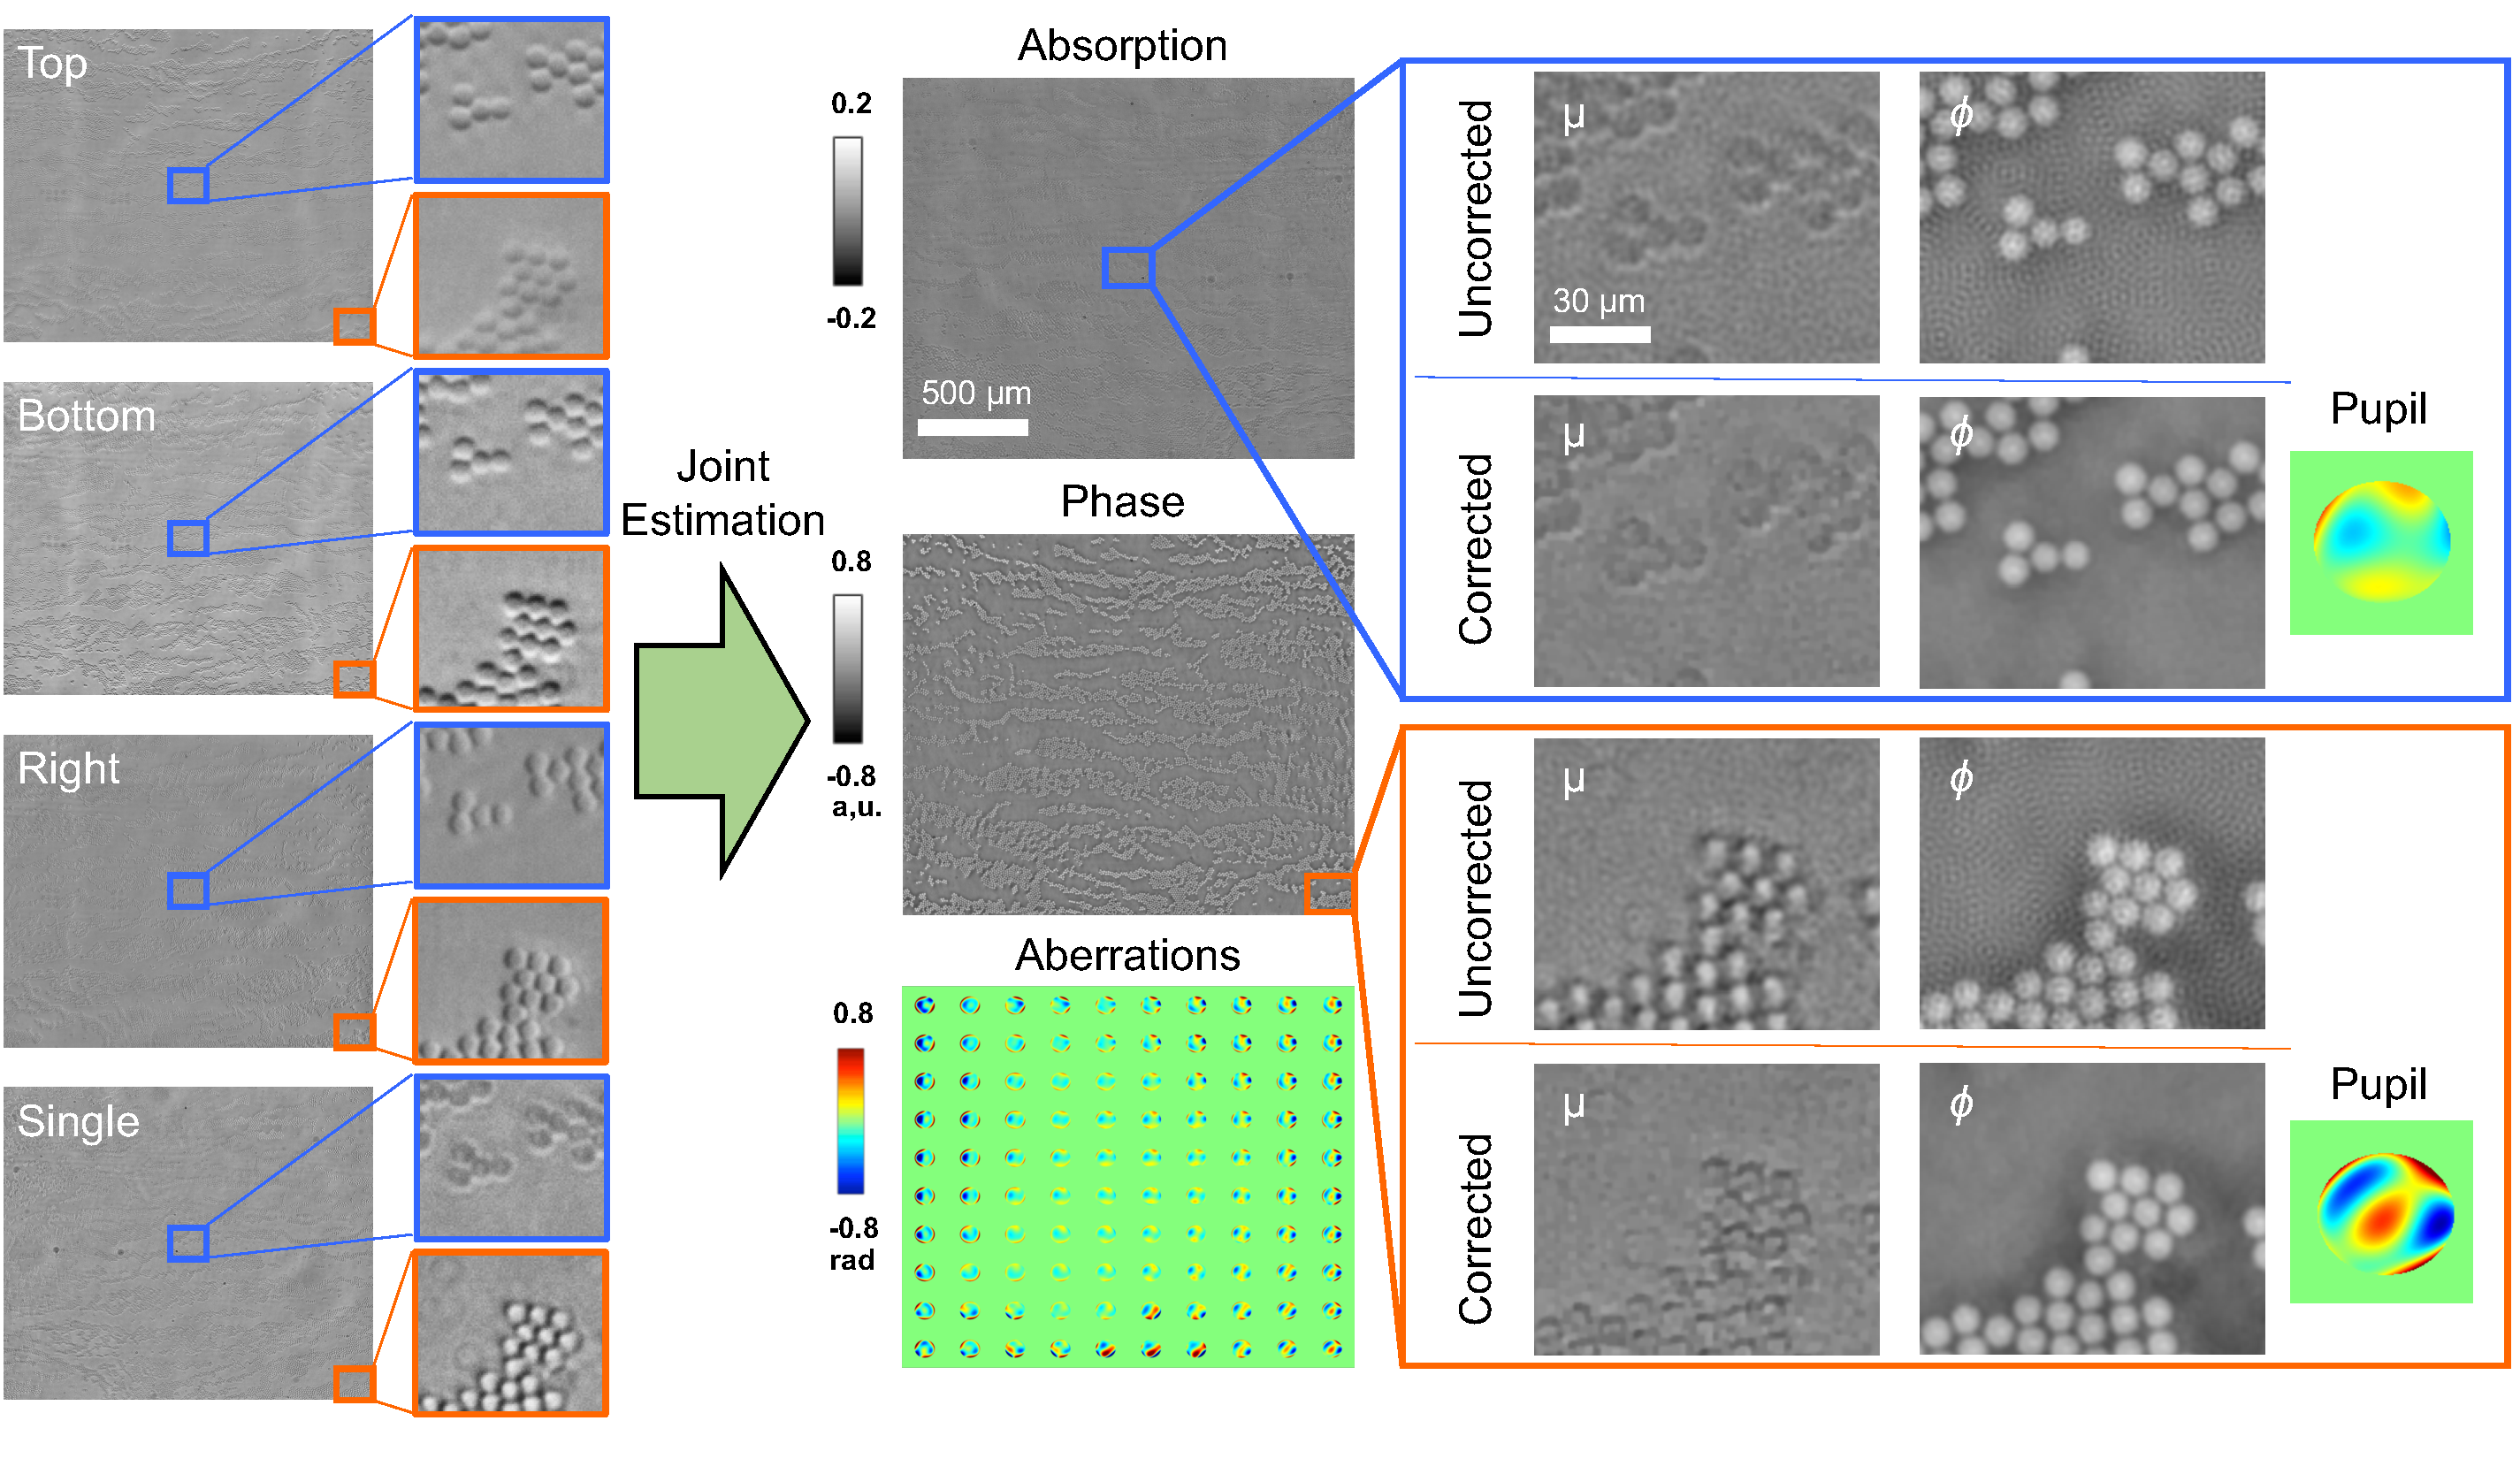
\includegraphics[width=1.0\textwidth]{fig_self_cal_dpc_results2.pdf}
\caption{\label{fig:self_cal_dpc_experimentalresults2} (a) Quantitative phase reconstructions of a USAF 1951 resolution target at various defocus distances with and without aberration correction, and the corresponding recovered aberrations (see Visualization 2). (b) Zoomed-in reconstructions at defocus of $10 \mu m$. (c) Known and experimentally-estimated defocus values from the $4^{th}$ Zernike mode over time.}
\end{figure}

Our method is easily extended to account for spatially-varying aberrations, simply by solving the joint estimation problem separately over different patches of the FOV. In order to visualize spatially-varying aberrations, we prepared oil (Cargille, $\mathrm{n}_{\mathrm{D}}=1.58$) immersed $10\mu m$ polystyrene beads (Sigma-Aldrich) as our sample, which is assumed to be nearly spatially invariant. The sample was imaged by a $4\times$ $0.2 \mathrm{NA}$ objective lens (Nikon, CFI Plan Apo Lambda) that has a FOV of 1.7 $\times$ 2.1mm. Four images were captured at 12.5Hz using the same source patterns as in Fig.~\ref{fig:self_cal_dpc_experimentalresults1}(a). Field-dependent aberrations are primarily caused by two types of system imperfections. First, the incident angle of individual LEDs changes from one FOV to another, since the relative position between the LEDs and the sample at each FOV varies. Second, thecd ..re exist spatially-varying aberrations native to the optical system. To accommodate this spatial variance, we break the full FOV into small patches, and apply the joint estimation algorithm on each patch independently. In this case, the incident angle of individual LEDs and the aberrations are assumed invariant within the patch, which is usually valid when the region is much smaller than the total FOV. In Fig.~\ref{fig:self_cal_dpc_experimentalresults3}(a), the full FOV is divided into 100 patches. Within each patch, the absorption, phase and pupil aberration were recovered independently before being stitched together to form the full FOV images. In practice, optimization for each patch converges in $20-30$ iterations.

Looking at the aberrations recovered, the center of the FOV is essentially aberration-free, which is consistent with the fact that optical systems are usually optimized there. Therefore, the absorption and phase images with pupil recovery are similar to that without aberration correction. Aberrations are much stronger along the edges of the FOV, where the field curvature blurs the image. Consequently, obvious differences occur between the normal DPC and aberration-corrected DPC reconstructions at those patches. The recovered amplitude (absorption) at the bottom right corner is dramatically changed after applying aberration correction. Qualitatively, the uncorrected absorption at the edge of the field appears to contain some phase information, leading to a shadow-like appearance; these artifacts are removed with pupil recovery. In addition, while aberrated phase evaluated with Tikhonov deconvolution suffered from high-frequency noise, phase with pupil correction shows reduced noise due to the use of TV regularization.

\begin{figure}[ht!]
\centering\includegraphics[width=0.9\textwidth]{fig_self_cal_dpc_results3.pdf}
\caption{\label{fig:self_cal_dpc_experimentalresults3} (a) Reconstructed absorption, phase and spatially-varying aberrations (recovered pupil wavefronts for different regions of the field-of-view). (b) Comparison of results with and without pupil estimation for central and edge regions of the field-of-view.}
\end{figure}

In computational imaging systems, system aberrations can significantly degrade quantitative phase and absorption reconstructions if not properly compensated. In order to correct the aberration without conducting additional measurements to calibrate the system, joint estimation of the sample and the pupil function is needed. While Fourier ptychography or coded aperture imaging provides pupil recovery, these methods often require many measurements. In this paper, we demonstrated a DPC-based phase retrieval technique that simultaneously recovers the system pupil function and quantitative phase and absorption of a sample with only 4 intensity images. By combining 3 DPC images as well as 1 measurement made under coherent illumination, diffraction-limited field and aberration with arbitrary Zernike orders were acquired through an alternating non-convex optimization. This method not only reduces the data acquisition time, but also increases signal-to-noise ratio due to higher light throughput compared to single-LED acquisition. The recovered system aberration are general to the system, and may be used for image correction in other imaging modalities, such as deconvolution of fluorescence images~\cite{Chung2016}.

\section{Source Self-Calibration using Fourier Ptychography}\label{sec:selfcal:fpm}

Computational imaging leverages the power of both optical hardware and computational algorithms to reconstruct images from indirect measurements. In optical microscopy, programmable sources have been used for computational illumination techniques including multi-contrast~\cite{Zheng2011,Liu2014}, quantitative phase~\cite{Zheng2013,Tian14,tian2015quantitative,Chen2016} and super-resolution~\cite{Zheng2013,ou2013quantitative,Dong:14,Tian2014}. Implementation is simple, requiring only an inexpensive source attachment for a commercial microscope. However, these methods are also sensitive to experimental misalignment errors and can suffer severe artifacts due to model mismatch. Extensive system calibration is needed to ensure that the inverse algorithm is consistent with the experimental setup, which can be time- and labor-intensive. This often requires significant user expertise, making the setup less accessible to reproduction by non-experts and undermining the simplicity of the scheme. Further, pre-calibration methods are not robust to changes in the system (e.g. bumping the setup, changing objectives, sample-induced aberrations) and require precise knowledge of a ground-truth test object.

Algorithmic self-calibration methods ~\cite{Thibault2009,Ou:14,Horstmeyer:14,Yeh2015,Sun:16LEDpos,Liu:17, maiden2012annealing, zhang2013translation,Bian:13,Bian:16,Dou2017,Eckert:16,Satat2016,Pan2017,Chung:16fluor} eliminate the need for pre-calibration and precise test objects by making calibration part of the inverse problem. These methods jointly solve two inverse problems: one for the reconstructed image of the object and the other for the calibration parameters. By recovering system calibration information directly from captured data, the system becomes robust to dynamic changes in the system.

\begin{figure*}[t]
	\centering
	\includegraphics[width=0.85\textwidth]{figures/fig_selfcal_fpm_overview.pdf}
	\caption{Illumination angles are calibrated by analyzing Fourier spectra. (a) A cheek cell is illuminated at angle $\alpha$ and imaged with $NA_{obj}$. (b) Brightfield images contain overlapping circles in their Fourier spectra; darkfield images do not. (c) We perform a fast and efficient brightfield calibration in pre-processing, then extrapolate the correction to darkfield images and, finally, iteratively calibrate angles inside the FPM algorithm using a spectral correlation calibration.
		}
	\label{fig:self_cal_fpm_overview}
\end{figure*}

Here, we focus on \textit{illumination angle} self-calibration for Fourier Ptychographic Microscopy (FPM)~\cite{Zheng2013}. FPM is a coherent computational imaging method that reconstructs high-resolution amplitude and phase across a wide field-of-view (FOV) from intensity images captured with a low-resolution objective lens and a dynamically-coded illumination source. Images captured with different illumination angles are combined computationally in an iterative phase retrieval algorithm that constrains the measured intensity in the image domain and pupil support in the Fourier domain. This algorithm can be described as stitching together different sections of Fourier space (synthetic aperture imaging~\cite{Turpin:1995,Di:08}) coupled with iterative phase retrieval. FPM has enabled fast \textit{in vitro} capture via multiplexing~\cite{Tian2014,tian2015quantitative}, fluorescence imaging~\cite{Chung:16fluor}, and 3D microscopy~\cite{tian20153d,Horstmeyer:16}. It requires significant redundancy (pupil overlap) in the dataset~\cite{Dong:14,Sun:16}, making it suitable for joint estimation self-calibration.

Self-calibration routines have previously been developed to solve for pupil aberrations~\cite{Thibault2009,Ou:14,Horstmeyer:14}, illumination angles~\cite{Yeh2015,Sun:16LEDpos,Liu:17, maiden2012annealing, zhang2013translation}, LED intensity~\cite{Bian:13}, sample motion~\cite{Bian:16}, and auto-focusing~\cite{Dou2017} in FPM. The state-of-the-art self-calibration method for illumination angles is simulated annealing~\cite{Yeh2015,Sun:16LEDpos}, a joint estimation solution which (under proper initialization) removes LED misalignment artifacts that usually manifest as low-frequency noise. Unfortunately, because the simulated annealing procedure operates inside the FPM algorithm iterative loop, it slows the run-time of the solver by an order of magnitude or more. For 3D FPM (which is particularly sensitive to angle calibration~\cite{tian20153d}), the computational costs become infeasible.

Moreover, most self-calibration algorithms require a relatively close initial guess for the calibration parameters. This is especially true when the problem is non-convex or if multiple calibration variables are to be solved for (\textit{e.g.} object, pupil, and angles of illumination). Of the relevant calibration variables for FPM, illumination angles are the most prone to error, due to shifts or rotations of the LED array~\cite{Guo:15}, source instabilities~\cite{Kuang:15,Eckert:16}, non-planar illuminator arrangements~\cite{Chung2016,phillips2015multi,Sen:16,Phillips:17}, or sample-induced aberrations~\cite{Hell:1993,Kang:18}. Sample-induced aberrations can also change the effective illumination angles dynamically, such as when the sample is in a moving aqueous solution.

We propose here a two-pronged angle self-calibration method that uses both pre-processing (\textit{brightfield calibration}) and iterative joint estimation (\textit{spectral correlation calibration}) that is quicker and more robust to system changes than state-of-the-art calibration methods\footnote{This work was developed in close collaboration with fellow Ph.D. student Regina Eckert (Waller Lab, EECS, UC Berkeley)}. A circle-finding step prior to the FPM solver accurately identifies the angles of illumination in the brightfield (BF) region. A transformation between the expected and BF calibrated angles extrapolates the correction to illuminations in the darkfield (DF) region. Then, a local grid-search-based algorithm inside the FPM solver further refines the angle estimates, with an optional prior based on the illuminator geometry (Fig.~\ref{fig:self_cal_fpm_overview}). Our method is object-independent, robust to coherent noise, and time-efficient, adding only seconds to the processing time. We demonstrate on-line angle calibration for 2D and 3D FPM with 3 different source types: an LED array, a galvanometer-steered laser, and a high-NA (max $NA_{illum} = 0.98$) quasi-dome illuminator~\cite{Phillips:17}.

\subsection{Methods}
The image formation process for a thin sample under off-axis spatially coherent plane wave illumination can be described by:
\begin{equation}
\vec{I}_i(\vec{r}) = |\vec{O}(\vec{r})e^{-i2\pi \vec{k}_i\vec{r}} * \vec{P}(\vec{r})|^2 = |\mat{F}^{-1}(\tilde{\vec{O}}(\vec{k}-\vec{k}_i)\tilde{\vec{P}}(\vec{k}))|^2,
\label{eq:forwardModel}
\end{equation}

\noindent where $\vec{k}_i$ is the spatial frequency of the incident light, $\tilde{\vec{P}}(\vec{k})$ is the system pupil function, $\tilde{\vec{O}}(\vec{k})$ is the object Fourier spectrum, and $\mat{F}$ is the 2D Fourier transformation operation, valid for shift-invariant systems. Intensity images are captured at the sensor plane, corresponding to auto-correlation in the Fourier domain:

\begin{equation}
\begin{split}
\tilde{\vec{I}}_i(\vec{k}) &= \mat{F}(|\vec{O}(\vec{r})e^{-i2\pi \vec{k}_i\vec{r}} * \vec{P}(\vec{r})|^2) \\
&=\tilde{\vec{O}}(\vec{k}-\vec{k}_i)\tilde{\vec{P}}(\vec{k}) \star \tilde{\vec{O}}(\vec{k}-\vec{k}_i)\tilde{\vec{P}}(\vec{k}),
\end{split}
\label{eq:Fourier domain}
\end{equation}

\noindent where $*$ denotes convolution and $\star$ denotes auto-correlation. $\tilde{\vec{O}}(\vec{k}-\vec{k}_i)\tilde{\vec{P}}(\vec{k})$ corresponds to the shifted spectrum of the object within the circle $|\vec{k}| \leq \frac{NA_{obj}}{\lambda}$ and 0 everywhere else. The auto-correlation operation essentially scans two copies of $\tilde{\vec{O}}(\vec{k}-\vec{k}_i)\tilde{\vec{P}}(\vec{k})$ across each other, coherently summing at each shift to give $\tilde{\vec{I}}_i(\vec{k})$. Typically, the object spectrum has a large zero-order (DC) term that decays sharply towards higher frequencies. In the brightfield region, when the DC term at $\vec{k}_i$ is within the pupil's passband, the auto-correlation effectively scans this DC term across the conjugate spectrum, giving high values where the DC term overlaps with the conjugate pupil and negligible signal elsewhere. This interference between the DC term and pupil in the auto-correlation creates two distinct circles centered at $\vec{k}_i$ and $-\vec{k}_i$ in the intensity spectrum amplitude (Fig.~\ref{fig:self_cal_fpm_overview}). Hence, we can calibrate the illumination angle by finding these circle centers. For darkfield images, the DC term is outside $\frac{NA_{obj}}{\lambda}$ and so we do not observe clearly defined circles in $|\tilde{\vec{I}}_i|$ (Fig.\ref{fig:self_cal_fpm_overview}b), making calibration more complicated.

Our algorithm relies on analysis of the raw intensity Fourier transform to recover illumination angles. Fourier domain analysis of intensity images has been used previously to deduce aberrations~\cite{Shanker:16} and determine the center of diffraction patterns~\cite{DAMMER1997214,CAUCHIE2008567} for system calibration. We show here that the individual Fourier spectra can be used to accurately determine illumination angles in both the brightfield and darkfield regime.

\subsection{Brightfield Calibration}
Locating the center of the circles in the amplitude of a Fourier spectrum is an image processing problem. Previous work in finding circles in images uses the Hough transform, which relies on an accurate edge detector as an initial step~\cite{Yuen89,Davies:04}. In practice, however, we find that edge detectors do not function well on our datasets due to speckle noise, making the Hough transform an unreliable tool for our purpose.

\begin{figure} [tb]
	\centering
	\includegraphics[width=0.6\textwidth]{figures/fig_selfcal_fpm_bf.pdf}
	\caption{Circular edge detection on brightfield images finds circle centers, giving illumination angle calibration. (a,b) Comparison of uncalibrated (red) and calibrated (black) illumination $\vec{k}_i$. The blue box in (b) indicates the search range for $\vec{k}_i$. (c,d) $\tilde{\vec{I}_i}$ along radial lines, $f(r,\phi_n)$, and derivatives with respect to $r$. (e,f) $\vec{E}_1$ and $\vec{E}_2$, sums of the derivatives at known radii $R$ and $R+\sigma$, peak near the correct center. Boxes show uncalibrated (red) and calibrated (black) $\vec{k}_i$ centers.
		}
	\label{fig:BF_calibration}
\end{figure}

Intuitively, circular edge detection can be understood as performing edge detection (\textit{i.e.} calculating image gradients) along a circular arc around a candidate center point in k-space (the Fourier domain). To first approximation, we assume $|\tilde{\vec{I}_i}|$ is a binary function that is 1 inside the two circles and 0 everywhere else. Our goal is to find the strong binary edge in order to locate the circle center.  We need only consider one of the circles, since the intensity image is real-valued and so its Fourier transform is symmetric. Based on information we have about our illumination set-up, we \textit{expect} the illumination spatial frequency (and therefore circle center) for spectrum $\tilde{\vec{I}_i}$ to be at $\vec{k}_{i,0} = (k_{x,i,0},k_{y,i,0})$ (polar coordinates $\vec{k}_{i,0} = (d_{i,0}, \theta_{i,0})$) (Fig.~\ref{fig:BF_calibration}a). If this is the \textit{correct} center  $\vec{k}_i'$, we expect there to be a sharp drop in $|\tilde{\vec{I}_i}|$ at radius $R$ along any radial line $f(r,\phi_n)$ out from $\vec{k}_i'$ (Fig.~\ref{fig:BF_calibration}b). This amplitude edge will appear as a peak at $r=R$ in the first derivative of each radial line with respect to $r$, $f'(r,\phi_n)$ (Fig.~\ref{fig:BF_calibration}d). Here $(r,\phi_n)$ are the polar coordinates of the radial line with respect to the center $\vec{k}_i$, considering the $n^{th}$ of $N$ radial lines.

We identify the correct $\vec{k}_i'$ by evaluating the summation of the first derivative around the circular arc at $r=R$ from several candidate $\vec{k}_i = (d_i,\theta_i)$ positions:

\begin{equation}
\vec{E}_1(R, d_i,\theta_i)=\sum_{n=1}^{N} f'(r = R,\phi_n,d_i,\theta_i).
\label{eq:eprime}
\end{equation}

\noindent When $\vec{k}_i$ is incorrect, the edges do not align and the derivative peaks do not add constructively at $R$ (Fig.~\ref{fig:BF_calibration}c). The derivatives at $R$ are all maximized \textit{only} at the correct center $\vec{k}_i'$ (Fig.~\ref{fig:BF_calibration}d), creating a peak in $\vec{E}_1$ (Fig.~\ref{fig:BF_calibration}e). This is analogous to applying a classic edge filter in the radial direction from a candidate center and accumulating the gradient values at radius $R$.

In order to bring our data closer to our binary image approximation, we divide out the average spectrum $\mathrm{mean}_i(|\tilde{\vec{I}_i}|)$ across all $i$ spectra. Because the object remains constant across images while the angles of illumination change, the average spectrum is similar in form to the object's auto-correlation spectrum, with a sharp central peak decaying towards higher frequencies. The resulting normalized spectra contain near-constant circles on top of background from higher-order terms. We then convolve with a Gaussian blur kernel with standard deviation $\sigma$ to remove speckle noise (Alg.~\ref{alg:BF}.\ref{alg:1}-\ref{alg:2}). Experi

mentally, we choose $\sigma = 2$ pixels, which balances blurring speckle noise and maintaining the circular edge. Under this model, the radial line $f(r,\phi_n)$ from our correct center $\vec{k}_i'$ can be modeled near the circular edge as a binary step function convolved with a Gaussian:

\begin{equation}
f(r,\phi_n,d_i',\theta_i') = \text{rect}(\frac{r}{2R}) * \frac{1}{\sqrt{2\pi}\sigma}e^{\frac{-r^2}{2\sigma^2}}.
\label{eq:spoke}
\end{equation}


\noindent By differentiating through $f'''(r,\phi_n)$ and setting equal to zero, we find the peak of $f'(r,\phi_n)$ still occurs at $r=R$. Additionally, we find that the second derivative $f''(r,\phi_n)$ has a maximum at $r=R+\sigma$. Experimentally, we have found that considering both the first \textit{and} second derivatives increases our accuracy and robustness to noise across a wide variety of datasets. We therefore calculate a second derivative metric,

\begin{equation}
\vec{E}_2(R+\sigma,d_i,\theta_i)=\sum_{n=1}^{N} f''(r = R+\sigma,\phi_n,d_i,\theta_i),
\label{eq:edoubleprime}
\end{equation}

\noindent which is jointly considered with Eq.~\ref{eq:eprime}. We identify candidate centers $\vec{k}_i$ that occur near the peak of \textit{both} $\vec{E}_1$ and $\vec{E}_2$ (Fig.~\ref{fig:BF_calibration}e-f), then use a least-squares error metric to determine the final calibrated $\vec{k}_i'$ (Alg.~\ref{alg:BF}.\ref{alg:5}-\ref{alg:8}). In practice, we also only consider the non-overlapping portion of the circle's edge, bounding $\vec{\phi}$.

Until now, we have assumed that the precise radius $R$ of the pupil is known. However, in pixel units, $R$ is dependent on the pixel size of the sensor, $p_s$, and the system magnification, $mag$:

\begin{equation}
R = \frac{NA_{obj}}{\lambda} \frac{p_s*M}{mag},
\end{equation}

\noindent as well as $NA_{obj}$ and $\lambda$, where $\tilde{\vec{I}_i}$ is dimension $M\times M$. Given that $mag$ and $NA_{obj}$ are often imprecisely known but are unchanged across all images, we calibrate the radius by finding the $R'$ which gives the maximum gradient peak $\vec{E}_1$ across multiple images before calibrating $\vec{k}_i'$ (Alg.~\ref{alg:BF}.\ref{alg:3}). A random subset of images may be used to decrease computation time.

\begin{algorithm}
\caption{Brightfield Calibration}\label{alg:BF}
\begin{algorithmic}[1]
\State $\tilde{\vec{I}}_f \gets |\tilde{\vec{I}}|/\textrm{mean}_i(|\tilde{\vec{I}_i}|)$\Comment{Divide out mean spectrum}\label{alg:1}
\State $\tilde{\vec{I}}_f \gets \textrm{gauss}(\tilde{\vec{I}}_f,\sigma)$\Comment{Smooth speckle}\label{alg:2}
\State $R' \gets \argmax_R \vec{E}_1(R,d_i,\theta_i), \textrm{subset }(\tilde{\vec{I}}_{f,i})$\Comment{Calibrate radius}\label{alg:3}
\For{$i^{th}$ image}
\Comment{Circular edge detection}
\State $\vec{k}_{i,1} \gets (d_i,\theta_i) \textrm{ where } \vec{E}_1 \textrm{ near max (within 0.1 std)}$\label{alg:5}
\State $\vec{k}_{i,2} \gets (d_i,\theta_i) \textrm{ where } \vec{E}_2 \textrm{ near max}$
\State $\vec{k}_{i} \gets \vec{k}_{i,1} \cap \vec{k}_{i,2}$\Comment{Consider both metrics}
\State $\vec{k}_i' \gets \argmin_{\vec{k}_i} ||\vec{I}_i - \mat{F}(\tilde{\vec{I}_i}\cdot\tilde{\vec{P}}(\vec{k}-\vec{k_i}))||_2$ \Comment{Evaluate $\vec{k}_i$}
\EndFor \label{alg:8}
\State $\mat{A}, i_{outliers} \gets \textrm{RANSAC}(\mat{A}=\vec{k}_i'/\vec{k}_{i,0})$\Comment{Identify outliers} \label{alg:9}
\State $\vec{k}_{inliers}^{(0)} \gets \vec{k}_{inliers}'$\Comment{Initialize for FPM}
\State $\vec{k}_{outliers}^{(0)} \gets \mat{A}\vec{k}_{outliers,0}$
\State $\vec{k}_{darkfield}^{(0)} \gets \mat{A}\vec{k}_{darkfield,0}$ \label{alg:12}

\end{algorithmic}
\end{algorithm}

\subsection{Spectral Correlation Calibration}
While the brightfield (BF) calibration method localizes illumination angles using intrinsic contrast from each measurement, this contrast is not present in high-angle (darkfield) measurements (Fig.~\ref{fig:self_cal_fpm_overview}b). Therefore, we additionally solve a more general joint estimation problem to refine the initialization provided by BF calibration, where the object $\vec{O}(\vec{r})$, pupil $\vec{P}(\vec{k})$, and illumination angles $\vec{k_i}$ are optimized within the FPM algorithm. At each inner iteration, we estimate the $i^{th}$ illumination angle by minimizing the FPM objective function with respect to illumination angle (Fig.~\ref{fig:DF_calibration}a). This step finds the relative k-space location of the current spectrum $\tilde{\vec{I}_i}$ relative to the overall object, providing an estimate $\vec{k}_i^{(m)}$ relative to the other illuminator angles $\vec{k}^{(m)}_j$, $j\neq i$. We call this the spectral correlation method because this optimization implicitly finds $\vec{k}_i^{(m)}$ which best aligns the $i^{th}$ spectrum with the estimated object spectrum $\tilde{\vec{O}}(\vec{k})^{(m)}$.

\begin{figure*}[hbt]
	\centering
	\includegraphics[width=0.97\textwidth]{figures/fig_selfcal_fpm_df.pdf}
	\caption{BF calibration uses a fast pre-processing step to estimate illumination angles, then SC calibration iteratively refines them within the FPM solver. (a) Algorithm block diagram, (b) uncalibrated (red) and BF + SC calibrated (green) illumination angle map. Insets are example search spaces, showing local convexity. (d) FPM convergence plot for different methods.
		}
	\label{fig:DF_calibration}
\end{figure*}

Unlike previous joint estimation methods~\cite{Yeh2015,Sun:16LEDpos}, we constrain $\vec{k}_i$ to exist on the k-space grid defined by the our image sampling. Our k-space resolution is band-limited by the size of the image patch, $\vec{s}=(s_x,s_y)$, across which the illumination can be assumed coherent. This coherent area size is determined by the van Cittert-Zernike theorem, which can be simplified~\cite{BornWolf} to show that the coherence length $l_c$ of illumination with mean source wavelength $\bar{\lambda}$ produced by a source of size $\rho$ at a distance $R$ is determined by:

\begin{equation}\label{eq:vancittert_zernike}
l_c = \frac{0.61 R \bar{\lambda}}{\rho}.
\end{equation}

\noindent For example, a $300\mu m$ wide LED placed $50 mm$ above the sample with $\bar{\lambda} = 530nm$ gives $l_c = 53.8\mu m$, which provides an upper bound on the size of image patch used in the FPM reconstruction, $(s_x,s_y) \leq l_c$. This limitation imposes a minimum resolvable discretization of illumination angles $\Delta{\vec{k}} = \frac{2}{\vec{s}}$ due to the Nyquist criterion. Since we cannot resolve finer angle changes, we need only perform a local grid search over integer multiples of $\Delta{\vec{k}}$, which makes our joint estimation SC method much faster than previous methods.

SC calibration is cast as an iterative optimization of discrete perturbations of the estimated angle using a local grid search. At each FPM iteration, we solve for the optimal perturbation of illumination angle  $\vec{{k}}_i^{(m)}$ over integer multiples $\vec{n} = (n_x, n_y)$ of k-space resolution-limited steps $\Delta \vec{k}$ such that the updated illumination position $\vec{k}_i^{(m+1)} = \vec{{k}}_i^{(m)} + \vec{n} \cdot \vec{\Delta {k}}$ minimizes the $\ell 2$ distance between the object and illumination angle estimates and measurements,

\begin{equation}\label{Eq:positionOpt}
    \begin{aligned}
    & \underset{\vec{n}}{\text{argmin}}
    & & ||\vec{I}_{i}- |\vec{O}^{(m+1)} e^{-i2\pi (\vec{{k}}_i^{(m)} + \vec{n} \Delta\vec{{k}})\vec{\vec{r}}} * \vec{P}^{(m+1)}|^2||_2^2 \\
    & \text{subject to}
    & &  \vec{n} = (n_x, n_y), \qquad (n_x, n_y) \in [-1, 0 ,1].
    \end{aligned}
\end{equation}

\noindent This grid search is performed iteratively within each sequential iteration of an FPM reconstruction until $\vec{k}_i$ converges, giving a lower reconstruction cost than BF calibration alone (Fig.~\ref{fig:DF_calibration}b-c).

The choice of $\vec{n} = (n_x, n_y)$ to search can be tuned to match the problem. In most experimental cases, we find that a search of the immediate locality of the current estimate ($(n_x, n_y) \in [-1, 0 ,1]$) gives a good balance between speed and gradient performance when paired with the close initialization from our BF calibration. A larger search range (e.g. $(n_x, n_y) \in [-2, -1, 0, 1, 2]$) may be required in the presence of noise or without a close initialization, but the number of points searched will increase with the square of the search range, causing the algorithm to slow considerably.



\begin{figure*} [htb]
	\centering
	\includegraphics[width=1\textwidth]{figures/fig_selfcal_fpm_mosaic.pdf}
	\caption{Experimental results with an LED array microscope, comparing reconstructions with no calibration (average reconstruction time 132 seconds), simulated annealing (3453 s), our BF calibration (156 s), and our BF + SC calibration (295 s). (a) Amplitude reconstructions of a USAF target in a well-aligned system. (b) Amplitude reconstructions of the same USAF target with a drop of oil placed on top of the sample to simulate sample-induced aberrations. (c) Phase reconstructions of a human cheek cell with computationally misaligned illumination, and (d) a Siemens star phase target with experimentally misaligned illumination.
		}
	\label{Fig:results}
\end{figure*}



Including prior information about the design of the illumination source can make our calibration problem more well-posed. For example, we can include knowledge that an LED array is a rigid, planar illuminator in our initial guess of the illumination angle map, $\vec{k}_{i,0}$. By forcing the current estimates $\vec{k}_i^{(m)}$ to fit a transformation of this initial angle map at the end of each FPM sub-iteration, we can use this knowledge to regularize our optimization (Fig.~\ref{fig:DF_calibration}a). The transformation model used depends on the specific illuminator. For example, our quasi-dome LED array is composed of five circuit boards with precise LED positioning within each board but variable board position relative to each other. Thus, imposing an affine transformation from the angle map of each board to the current estimates $\vec{k}_i^{(m)}$ significantly reduces the problem dimensionality and mitigates noise across LEDs, making the reconstruction more stable.

\subsection{Results}

\begin{figure*} [t]
	\centering
	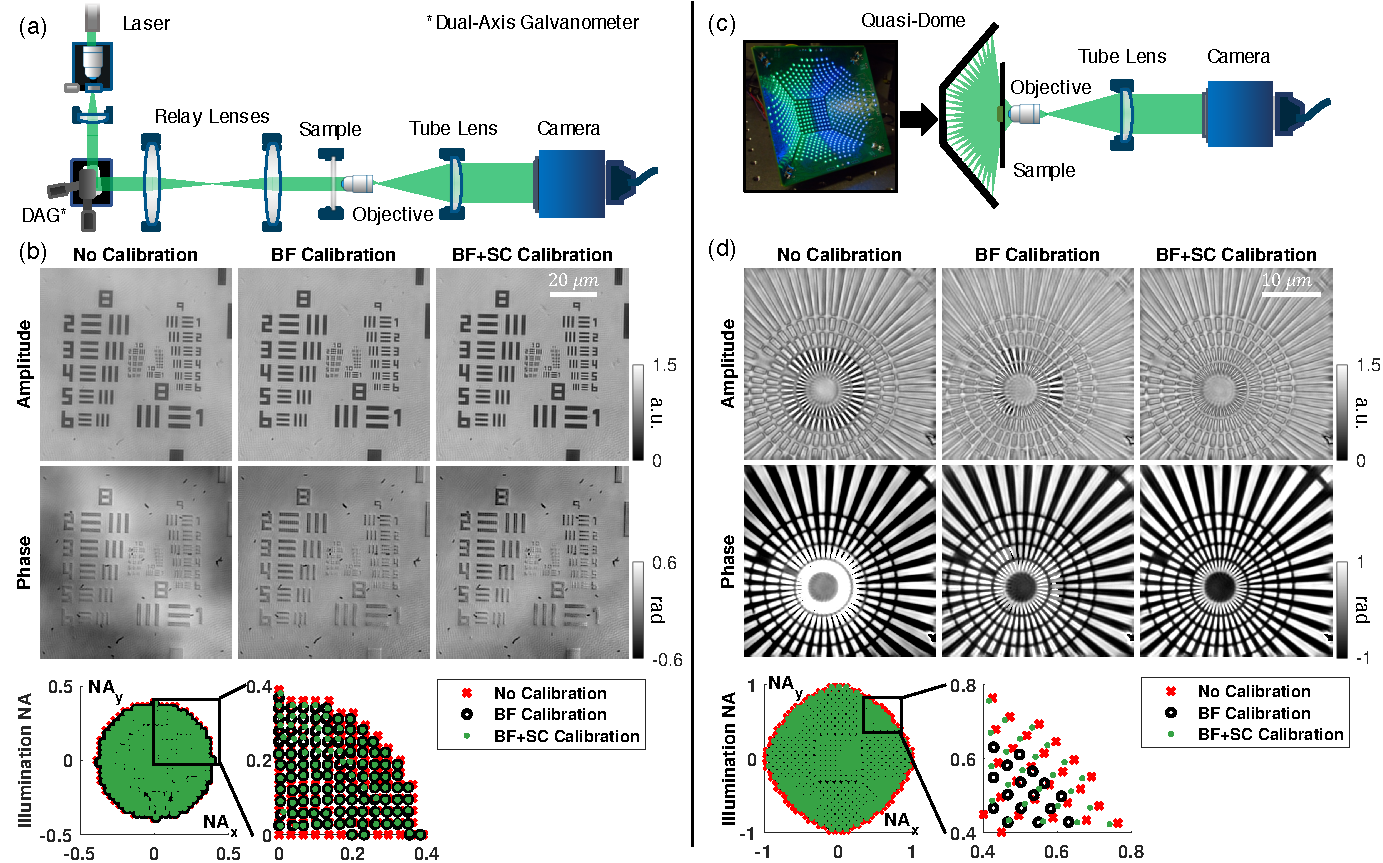
\includegraphics[width=1\textwidth]{figures/fig_selfcal_fpm_system.pdf}
	\caption{Experimental angle calibration in laser and high-NA quasi-dome illumination systems. (a) Laser illumination is steered by a dual-axis galvanometer. The angled beam is relayed to the sample by 4", 80 mm focal length lenses. (b) Our calibration method removes low-frequency reconstruction artifacts. (c) The quasi-dome illuminator enables up to 0.98 $NA_{illum}$ using programmable LEDs. (d) Our 1.23 NA reconstruction provides isotropic 425 $nm$ resolution with BF + SC calibration.
		}
	\label{Fig:laserDome}
\end{figure*}

\subsubsection{Planar LED Array}
We first show experimental results from a conventional LED array illumination system with a 10$\times$, 0.25 NA and a 4$\times$, 0.1 NA objective lens at $\lambda = 514 nm$ and $NA_{illum} \leq 0.455$ (Fig.~\ref{Fig:results}). We compare reconstructions with simulated annealing, our BF pre-processing alone, and our combined BF+SC calibration method. All methods were run in conjunction with EPRY pupil reconstruction~\cite{Ou:14}. We include results with and without the SC calibration to illustrate that the BF calibration is sufficient to correct for most misalignment of the LED array since we can accurately extrapolate LED positions to the darkfield region when the LEDs fall on a planar grid. However, when using a low NA objective ($NA_{obj} \leq 0.1$), as in Fig.~\ref{Fig:results}d, the SC method becomes necessary because the BF calibration is only able to use 9 images (compared to 69 brightfield images with a 10$\times$, 0.25 NA objective, as in Fig.~\ref{Fig:results}a-c).

Our method is object-independent, so can be used for phase and amplitude targets as well as biological samples. All methods reconstruct similar quality results for the well-aligned LED array with the USAF resolution target (Fig.~\ref{Fig:results}a). To simulate an aqueous sample, we place a drop of oil on top of the resolution target. The drop causes uneven changes in the illumination, giving low-frequency artifacts in the uncalibrated and simulated annealing cases which are corrected by our method (Fig.~\ref{Fig:results}b). Our method is also able to recover a $5^{\circ}$ rotation, 0.02 NA shift, and 1.1$\times$ scaled computationally-imposed misalignment on well-aligned LED array data for a cheek cell (Fig.~\ref{Fig:results}c), and gives a good reconstruction of an experimentally misaligned LED array for a phase Siemens star (Benchmark Technologies, Inc.) (Fig.~\ref{Fig:results}d). In contrast to simulated annealing, which on average takes $26 \times$ as long to process as FPM without calibration, our brightfield calibration only takes an additional 24 seconds of processing time and the combined calibration takes roughly only $2.25 \times$ as long as no calibration.

\subsubsection{Steered Laser}
Laser illumination can be used instead of LED arrays to increase the coherence and light efficiency of FPM~\cite{Kuang:15,Chung2016}. In practice, laser systems are typically less rigidly aligned than LED arrays, making them more difficult to calibrate. To verify the performance of our method, we constructed a laser-based FPM system using a dual-axis galvanometer to steer a 532 $nm$, 5 mW laser, which is focused on the sample by large condenser lenses (Fig.~\ref{Fig:laserDome}a). This laser illumination system allows finer, more agile illumination control than an LED array, as well as higher light throughput. However, the laser illumination angle varies from the expected value due to offsets in the dual-axis galvonometer mirrors, relay lens aberrations, and mirror position mis-estimations when run at high speeds. Our method can correct for these problems in a fraction of the time of previous methods (Fig.~\ref{Fig:laserDome}b).

\subsubsection{Quasi-Dome}

Since the FPM resolution limit is set by $NA_{obj} + NA_{illum}$, high-NA illuminators are needed for large space-bandwidth product imaging~\cite{Sun2017,Phillips:17}. To achieve high-angle illumination with sufficient signal-to-noise ratio in the darkfield region, the illuminators must become more dome-like, rather than planar~\cite{phillips2015multi}. We previously developed a novel programmable quasi-dome array made of five separate planar LED arrays that can illuminate up to 0.98 NA~\cite{Phillips:17}. This device uses discrete LED control with RGB emitters ($\bar{\lambda}=[475nm, 530nm, 630nm]$) and can be easily attached to most commercial inverted microscopes (Fig.~\ref{Fig:laserDome}c).

As with conventional LED arrays, we assume that the LEDs on each board are rigidly placed as designed. However, each circuit board may have some relative shift, tilt, or rotation since the final mating of the 5 boards is performed by hand. LEDs with high-angle incidence are both harder to calibrate and more likely to suffer from mis-estimation due to the dome geometry, so the theoretical reconstruction NA would be nearly impossible to reach without self-calibration. Using our method, we obtain the theoretical resolution limit available to the quasi-dome (Fig.~\ref{Fig:laserDome}d). The SC calibration is especially important in the quasi-dome case since it usually has many darkfield LEDs.

\subsection{Discussion}
\begin{figure} [t]
	\centering
	\includegraphics[width=0.5\textwidth]{figures/fig_selfcal_fpm_accuracy.pdf}
	\caption{Our calibration methods are robust to large mismatches between estimated and actual LED array position. Simulation of misaligned illumination by (a) rotation, (b) shift, and (c) scale. Our calibration recovers the illumination with <0.005 NA error for rotations of $-45^{\circ}$ to $45^{\circ}$, shifts of -0.1 to 0.1 NA, and scalings of 0.5$\times$ to 1.75$\times$ before diverging.
		}
	\label{Fig:self_cal_fpm_accuracy}
\end{figure}

Our calibration method offers significant gains in speed and robustness as compared to previous methods. BF calibration enables these capabilities by obtaining a good calibration that needs to be calculated only once in pre-processing, reducing computation. Since an estimation of a global shift in the illuminator based only on the brightfield images provides such a close initialization for the rest of the illumination angles, we can use a quicker, easier joint estimation computation in our SC calibration than would be otherwise possible. Jointly, these two methods work together to create fast and accurate reconstructions.

We analyze the robustness of our method to illumination changes by simulating an object illuminated by a grid of LEDs with $NA_{illum}<0.41$, with LEDs spaced at $0.041 NA$ intervals. We define the system to have $\lambda = 532 nm$, with a 10$\times$, 0.25 NA objective, a 2$\times$ system magnification, and a camera with $6.5 {\mu}m$ pixels. While the actual illumination angles in the simulated data remain fixed, we perturb the expected angle of illumination in typical misalignment patterns for LED arrays: rotation, shift, and scale (analogous to LED array distance from sample). We then calibrate the unperturbed data with the perturbed expected angles of illumination as our initial guess.

Our method recovers the actual illumination angles with error less than 0.005 NA for rotations of $-45^{\circ}$ to $45^{\circ}$ (Fig.~\ref{Fig:self_cal_fpm_accuracy}a); shifts of -0.1 to 0.1 NA, or approximately a displacement of +/- 2 LEDs (Fig.~\ref{Fig:self_cal_fpm_accuracy}b); and scalings of 0.5$\times$ to 1.75$\times$ (or LED array height between 40-140 $cm$ if the actual LED array height is 70 $cm$) (Fig.~\ref{Fig:self_cal_fpm_accuracy}c). In these ranges, the average error is 0.0024 NA, less than the k-space resolution of 0.0032 NA. Hence, our calibrated angles are very close to the actual angles even when the input expected angles are extremely far off. This result demonstrates that our method is robust to most mis-alignments in the illumination scheme.

In summary, we have presented a novel two-part calibration method for recovering the illumination angles of a computational illumination system for Fourier ptychography. We have demonstrated how this self-calibrating method makes Fourier ptychographic microscopes more robust to system changes and aberrations introduced by the sample. The method also makes it possible to use high-angle illuminators, such as the quasi-dome, and non-rigid illuminators, such as laser-based systems, to their full potential. Our pre-processing brightfield calibration further enables 3D multislice Fourier ptychography to reconstruct high-resolution features across larger volumes than previously possible. These gains were all made with minimal additional computation, especially when compared to current state-of-the-art methods. Efficient self-calibrating methods such as these are important to make computational imaging methods more robust and available for broad use in the future.

\section{Summary}

In computational imaging systems, mis-calibrations can significantly degrade reconstructions if not properly compensated for. Here, we have presented two frameworks for algorithmic self-calibration. In Section~\ref{sec:selfcal:dpc}, we presented a novel method for performing self-calibration of system aberrations using just four measurements - three half-circle (DPC) measurements and one coherent (single-LED) measurement. These four measurements enable the recovery of \textit{both} the compelx field of the object as well as spatially-varinat system aberrations. These aberrations can be acquired quickly and reconstructed using standard reconstruction techniques such as ADMM. In Section~\ref{sec:selfcal:fpm}, we presented a novel method for recovering source illumination angles of planar, quasi-domed, and steered laser sources using an offline (image-based) self-calibration algorithm, which is then refined using an online (FPM-based) self-calibration algorithm. For devices subject to manufacturing variations (such as the quasi-dome), these techniques are absolutely essential for high-resolution FPM reconstructions.

Owing to their non-convex formulations, self-calibration will never be as good as proper physical calibration of the systems, when such calibration is possible. However, when mis-calibration is suspected, these methods will always improve reconstruction quality compared to the uncorrected case, and therefore should be used whenever possible. Practically, the performance Quasi-dome presented in Section~\ref{sec:fabrication:quasidome} is significantly improved using self-calibration due to positioning error between printed circuit boards it is composed of. The open-source code used in these sections is provided in the Appendix~\ref{ch:appendix}, Section~\ref{sec:appendix:opensource}.
